\utsection{OpenBSC}{Stefan Giggenbach}\label{sec:openbsc}

\subsection{Überblick}

Bei OpenBSC handelt es sich wie bei OpenBTS um ein Open Source Projekt. Die Entwicklung erfolgt vollständig in der Sprache C und hat keinen direkten Bezug zum OpenBTS Projekt. Der große Vorteil von OpenBSC liegt in der \textit{network in the box} (nitb) genannten Version, die ohne zusätzliche Software-Komponenten den Betrieb eines GSM-Netzwerks ermöglicht. Mit OpenBSC wird zu einem sehr frühen Zeitpunkt im Projekt ein GSM-Netzwerk mit Handover-Funktionalität betrieben mit dem die entsprechenden Abläufe analysiert werden können (siehe Kapitel \ref{sec:analyse}).

\begin{figure}[h!]
  \centering
  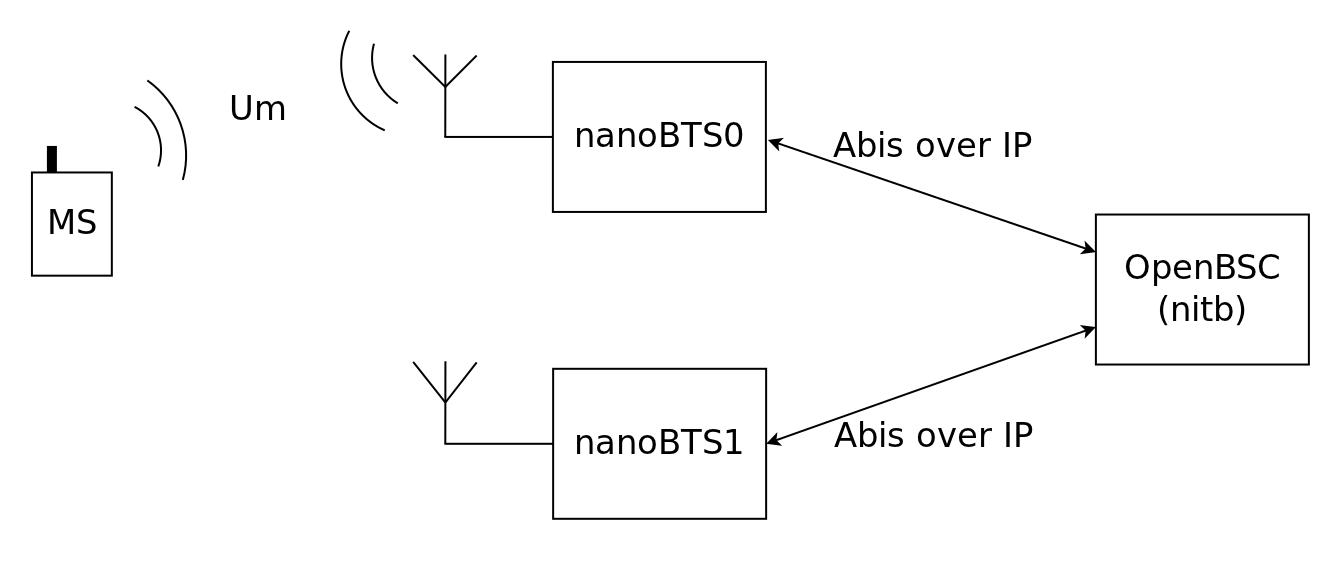
\includegraphics[width=0.9\textwidth]{img/openbscarch}
  \caption{OpenBSC Versuchsaufbau}
  \label{fig:openbscarch}
\end{figure}

Abbildung \ref{fig:openbscarch} zeigt den im Projekt verwendeten Versuchsaufbau. OpenBSC übernimmt nicht nur die Aufgaben des BSC, sondern auch die des MSC. Die Teilnehmerdatenbanken HLR und VLR werden mit einer SQLite3 Datenbank realisiert. Wie in Abbildung \ref{fig:openbscarch} dargestellt, werden zwei nanoBTS der Firma ip.access verwendet. Diese werden über getrennte Abis-over-IP-Schnittstellen an OpenBSC angebunden. Mit dem dargestellten Versuchsaufbau ist somit die Durchführung eines in Abschnitt \ref{sec:handover} beschriebenen Intra BSC Handover mit verhältnismäßig geringem Installations- und Konfigurationsaufwand möglich.

\subsection{Installation und Konfiguration}

Die Installation von OpenBSC ist ausführlich im Wiki des Projekts \cite{bib:buildopenbsc} dokumentiert. In diesem Abschnitt werden nur die wichtigsten Punkte der Installation und die Konfiguration des Systems für den Multi-BTS-Betrieb behandelt.

OpenBSC (nitb) besteht aus insgesamt drei Komponenten:

\begin{itemize}
 \item \textit{libosmocore} - Die Kernbibliothek, die auch für andere Projekte (z.\,B. OsmoBTS) verwendet wird.
 \item \textit{libosmo-abis} - Die Bibliothek zur Umsetzung der Abis- und Abis-over-IP-Schnittstellen.
 \item \textit{openbsc} - Die eigentliche OpenBSC-Software, welche auch die nitb Version enthält.
\end{itemize}

Nach der Kompilierung und Installation dieser drei Komponenten können die beiden nanoBTS, die sich im selben IP-Netzwerk befinden müssen, konfiguriert werden. Dazu werden die zwei Anwendungen \lstinline{./ipaccess-find} und \lstinline{./ipaccess-config} im Verzeichnis \lstinline{<openbsc>/src/ipaccess} benötigt. Die Verwendung der beiden Anwendungen und die benötigten Parameter zur Konfiguration werden ebenfalls im Wiki des Projekts \cite{bib:ipaccess} erläutert. Die bei der Konfiguration der nanoBTS vergebene UnitID wird dabei für die im Folgenden beschriebene Konfiguration von OpenBSC benötigt.

Um den Betrieb beider nanoBTS und die Handover-Funktionalität von OpenBSC zu aktivieren, muss die Konfigurationsdatei von OpenBSC modifiziert werden. Als Grundlage wird die Beispielkonfiguration \lstinline{<openbsc>/doc/examples/osmo-nitb/nanobts/openbsc.cfg} verwendet. Listing \ref{lst:config} zeigt auszugsweise die wichtigsten Inhalte der modifizierte Konfigurationsdatei.

\begin{lstlisting}[label=lst:config,caption=OpenBSC Konfigurationsdatei (Auszug)]
!
! OpenBSC (0.10.1.40-2935) configuration saved from vty
.
network
 network country code 262
 mobile network code 98
 .
 handover 1
 .
 bts 0
  type nanobts
  band DCS1800
  cell_identity 0
  .
  ip.access unit_id 42 0
  .
  trx 0
   rf_locked 0
   arfcn 846
   nominal power 23
   max_power_red 22
   .
 bts 1
  type nanobts
  band DCS1800
  cell_identity 1
  .
  ip.access unit_id 43 0
  .
  trx 0
   rf_locked 0
   arfcn 867
   nominal power 23
   max_power_red 22
   .
\end{lstlisting}

Neben dem Network Country Code und dem Mobile Network Code (Zeilen 5 und 6) muss in den Netzwerkeinstellungen die Handover-Funktionalität gesetzt werden (Zeile 8). Die Konfiguration der beiden nanoBTS beschränkt sich im Wesentlichen auf die Vergabe der eindeutigen CellIDs (Zeilen 13 und 26), der vorher festgelegten UnitIDs (Zeilen 15 und 28) und den beiden Frequenzen (ARFCN in Zeilen 19 und 32).

Nach der Modifikation der Konfigurationsdatei wird diese im Verzeichnis \lstinline{<openbsc>/src/osmo-nitb} gespeichert. Anschließend kann das System mit dem Befehl \lstinline{./openbsc} im selben Verzeichnis gestartet werden. Die Bedienung von OpenBSC erfolgt nach dem Start über eine Telnetsitzung auf Port 4242. Mit Hilfe des Command Line Interfaces der Telnetsitzung ist auch die Administration der Teilnehmerdatenbank möglich. Die Verwendung des CLI ist aufgrund der interaktiven Eingabe selbsterklärend.

Um einen Handover auszulösen, kann bei aktiver Verbindung entweder die Position einer Mobile Station verändert werden oder die Signalqualität wird durch entsprechende Schirmung der Geräte in ausreichendem Umfang reduziert. Die Analyse der mit OpenBSC durchgeführten Handover wird in Kapitel \ref{sec:analyse} detailliert beschrieben.
